\documentclass[11pt]{article}
\usepackage{acl2015}
\usepackage{amsmath,amsfonts}
\usepackage{times}
\usepackage{url}
\usepackage{color}
\usepackage{latexsym}
\usepackage{epsfig}
\usepackage{subfig}
\usepackage{graphicx}
%\usepackage[pdftex]{graphicx}
%\DeclareGraphicsExtensions{.pdf,.jpeg,.png}
%\usepackage{epstopdf}
\usepackage{booktabs}
\usepackage{diagbox}
\usepackage{array}
\usepackage{multicol}
\usepackage{threeparttable}

\newcommand{\figref}[1]{Figure \ref{#1}}
\newcommand{\tabref}[1]{Table \ref{#1}}

\newcolumntype{I}{!{\vrule width 1pt}}
\newlength\savedwidth
\newcommand\whline{\noalign{\global\savedwidth\arrayrulewidth
                            \global\arrayrulewidth 1pt}%
                   \hline
                   \noalign{\global\arrayrulewidth\savedwidth}}
\newlength{\Oldarrayrulewidth}
\newcommand{\Cline}[2]{%
  \noalign{\global\setlength{\Oldarrayrulewidth}{\arrayrulewidth}}%
  \noalign{\global\setlength{\arrayrulewidth}{#1}}\cline{#2}%
  \noalign{\global\setlength{\arrayrulewidth}{\Oldarrayrulewidth}}}

\newcommand\norm[1]{\left\lVert#1\right\rVert}
\DeclareMathOperator*{\argmin}{arg\,min}

\newcommand{\KZ}[1]{\textcolor{blue}{Kenny: #1}}
\newcommand{\YZ}[1]{\textcolor{yellow}{Yizhong: #1}}

%\setlength\titlebox{5cm}

% You can expand the titlebox if you need extra space
% to show all the authors. Please do not make the titlebox
% smaller than 5cm (the original size); we will check this
% in the camera-ready version and ask you to change it back.


\title{ActionNews: Searching for News with Actions}

\author{Xinyu Hua \and Yifan Wang \and Yu Gong \and Kenny Q. Zhu  \\
  Shanghai Jiao Tong University \\
  {\tt \{huaxinyu,racheter,kenzhu\}@sjtu.edu.cn} \\
  }

\date{}

\begin{document}
\maketitle
\begin{abstract}
The system we propose aims to improve search accuracy for 
conceptual queries that contain actions, 
such as ``company buy company''.
We construct an action-noun mapping to abstract action triples 
by one or multiple single nouns. With this mapping, we are able 
to expand the user's query by its noun abstraction, 
in hope of retrieving more relevant documents without the explicit 
occurrence of the original terms in the query. 
%We model the relation between action concepts and
%noun abstractions as a special Tripartite graph, 
%with intermediate nodes representing 
%news articles as evidence of the relationship. 
We demonstrate our system as a news search engine which returns and
compares the results from our method, a baseline approach, 
as well as the default keyword search. 
\end{abstract}

\section{Introduction}

Protein$-$protein interactions (PPIs) are of central importance for the majority of biological functions, such as signal transduction, metabolic pathways, molecular dynamics, and protein networks\cite{Hoffmann.Krallinger.ea:2005}, for they serve as the most fundamental building blocks of the entire interacademic systems of any organisms. Collecting data on pairwise interaction relationships is essential for multiple purpose, including identification of modules with certain functionality\cite{Spirin.Mirny.03}, mapping diseases to dominated genes\cite{Ideker.Sharan.08}, and after all, understanding wholistic metabolic/genetic networks from a system biology perspective.

A lot of databases have been built to store protein and genetic interactions from major model organism species and are available in various standardized formats, such as MINT\cite{Zanzoni.Montecchi-Palazzi.ea:2002}, BIND\cite{Bader.ea:2003}, BIOGRID\cite{DBLP:journals/nar/StarkBRBBT06}, etc. Among those mainstream databases, the data largely rely on voluntary reports by scientists or researchers, besides, comprehensive curation efforts become indispensable for the sake of accuracy. However, the amount of biology-related literatures with respect to protein interactions grows explosively and thus make it either impossible or impractical to manually detect PPI information anymore.

Considering huge amount of PPI information with great wealth hidden in published papers, in recent years, numerous mining techniques have been proposed that aim to extract PPI information automatically from free text, especially machine learning, information retrieval, and natural language processing\cite{DBLP:journals/bib/WinnenburgWPDS08}.These approaches can be roughly categorized into three classes: co$-$occurrence, rule$-$based, and machine learning. 

Co$-$occurrence is the approach with most simplicity and naivete. Just as its name implies, this method intends to find out pairs of proteins that co-occur in the same context. The scope of "same context" ranges from phrase, sentence, paragraph to whole abstract, even document. The underlying assumption is that whenever two proteins are mentioned together by authors, chances are high that there is some kind of relationship between them. However, however, in-context closeness even semantic relation does not necessarily represent actual biological interaction. As a consequence, a large fraction of candidate pairs are mismatched inevitably, causing a high recall but low precision.

The second approach is rule-based extraction, in other words, pattern matching. There are many types of rules, most of them concern natural language processing (NLP). One way is to specify hand-crafted regular expressions before hand, which mostly lean on language usage preference. Besides, by using full or partial (shallow) parsing strategies, more information would be acquired, such as part-of-speech taggers, local dependencies between syntactic components, context-free grammar\cite{DBLP:journals/bioinformatics/TemkinG03}, and full sentence structure. Compared to co$-$occurrence, rule-based approach enjoy better precision but much lower recall. In addition, since the rules are usually derived from training data, that is to say, the improper choice of training data would be significantly lethal, therefore quality of extraction is invariably instable and may not applicable to other data.

The third and most commonly used approach use machine learning techniques, in this case, the task to extract protein$-$protein interactions turns out to be a binary classification problem. Each protein pairs are represented along with a set of features, which is associated with their context, then a well$-$defined classifier gives the answer whether the candidate protein pairs is classified to be qualified PPI. (TO BE FURTHER FILLED!!!)

In this paper, we introduce a general bootstrapping framework for Protein$-$protein interaction extraction from natural text.Our method differs from most of the previous works in three aspects:

(1)The extraction process is driven by only tiny fraction of training data, which are regarded as seed data. In each round, it would derive reliable patterns automatically from seed data, then extract more positive PPI pairs consequently, what's more, the seed data would be augmented by the newly extracted results with high confidence.

(2)multiple graph kernel. 

(3)various evaluation.





%\subsection{Model Overview}

In this section, we describe our joint model for cross-lingual table linking.
%\figref{fig:overview} gives a general view of our neural network based joint model.
\figref{fig:overview} gives a general view of the model.
The reason we call it a ``joint model'' is that
the input of neural network is a mention table $X$ containing all the cells to be linked,
together with one candidate entity table $E$,
%All the mentions in the table will be linked simultaneously.
and the output stands for the relevance score $S(X, E)$.
%which indicates the probability of choosing that candidate entity table as final result.

Specifically, we first generate candidate entities of each single mention (\secref{sec:candgen}),
then we learn two different features:
the \textbf{m}ention feature and \textbf{c}ontext feature
derived from the mention-entity embedding pairs of the table (\secref{sec:cell}).
To make different representations from two language spaces compatible,
we utilize a bilingual translation matrix to transform the vector representation
from Chinese to English (\secref{sec:translation}).
Meanwhile, we learn a third feature called \textbf{coh}erence feature
only from the candidate entity table (\secref{sec:coherence}).
%We combine these three features together to calculate the overall relevance score, and finally
Finally, we discuss the prediction and parameter learning step of this task (\secref{sec:strategy}). 

\begin{figure*}
	\centering
	%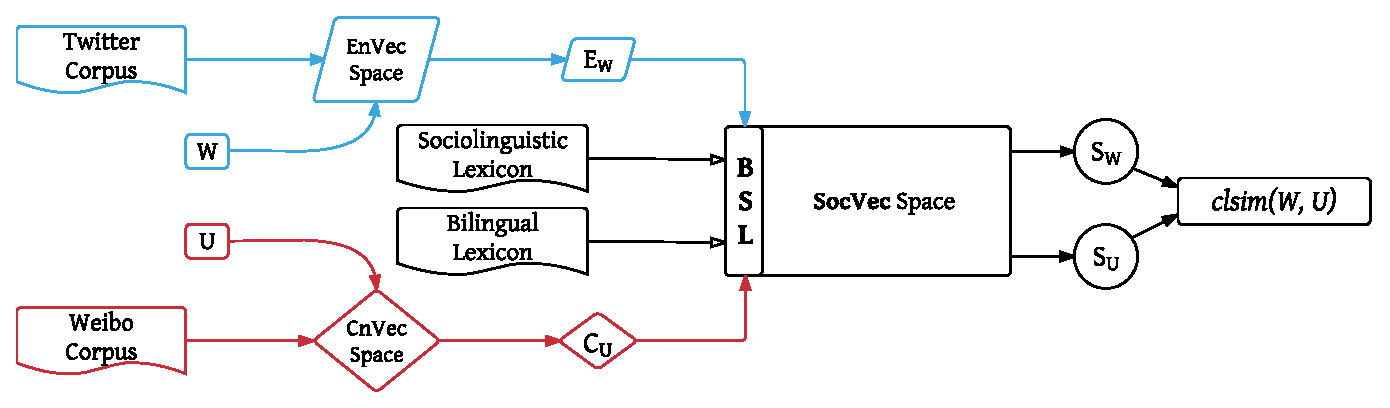
\epsfig{file=figures/overview.eps, angle=0, width=2.0\columnwidth}
	\scalebox{0.28}{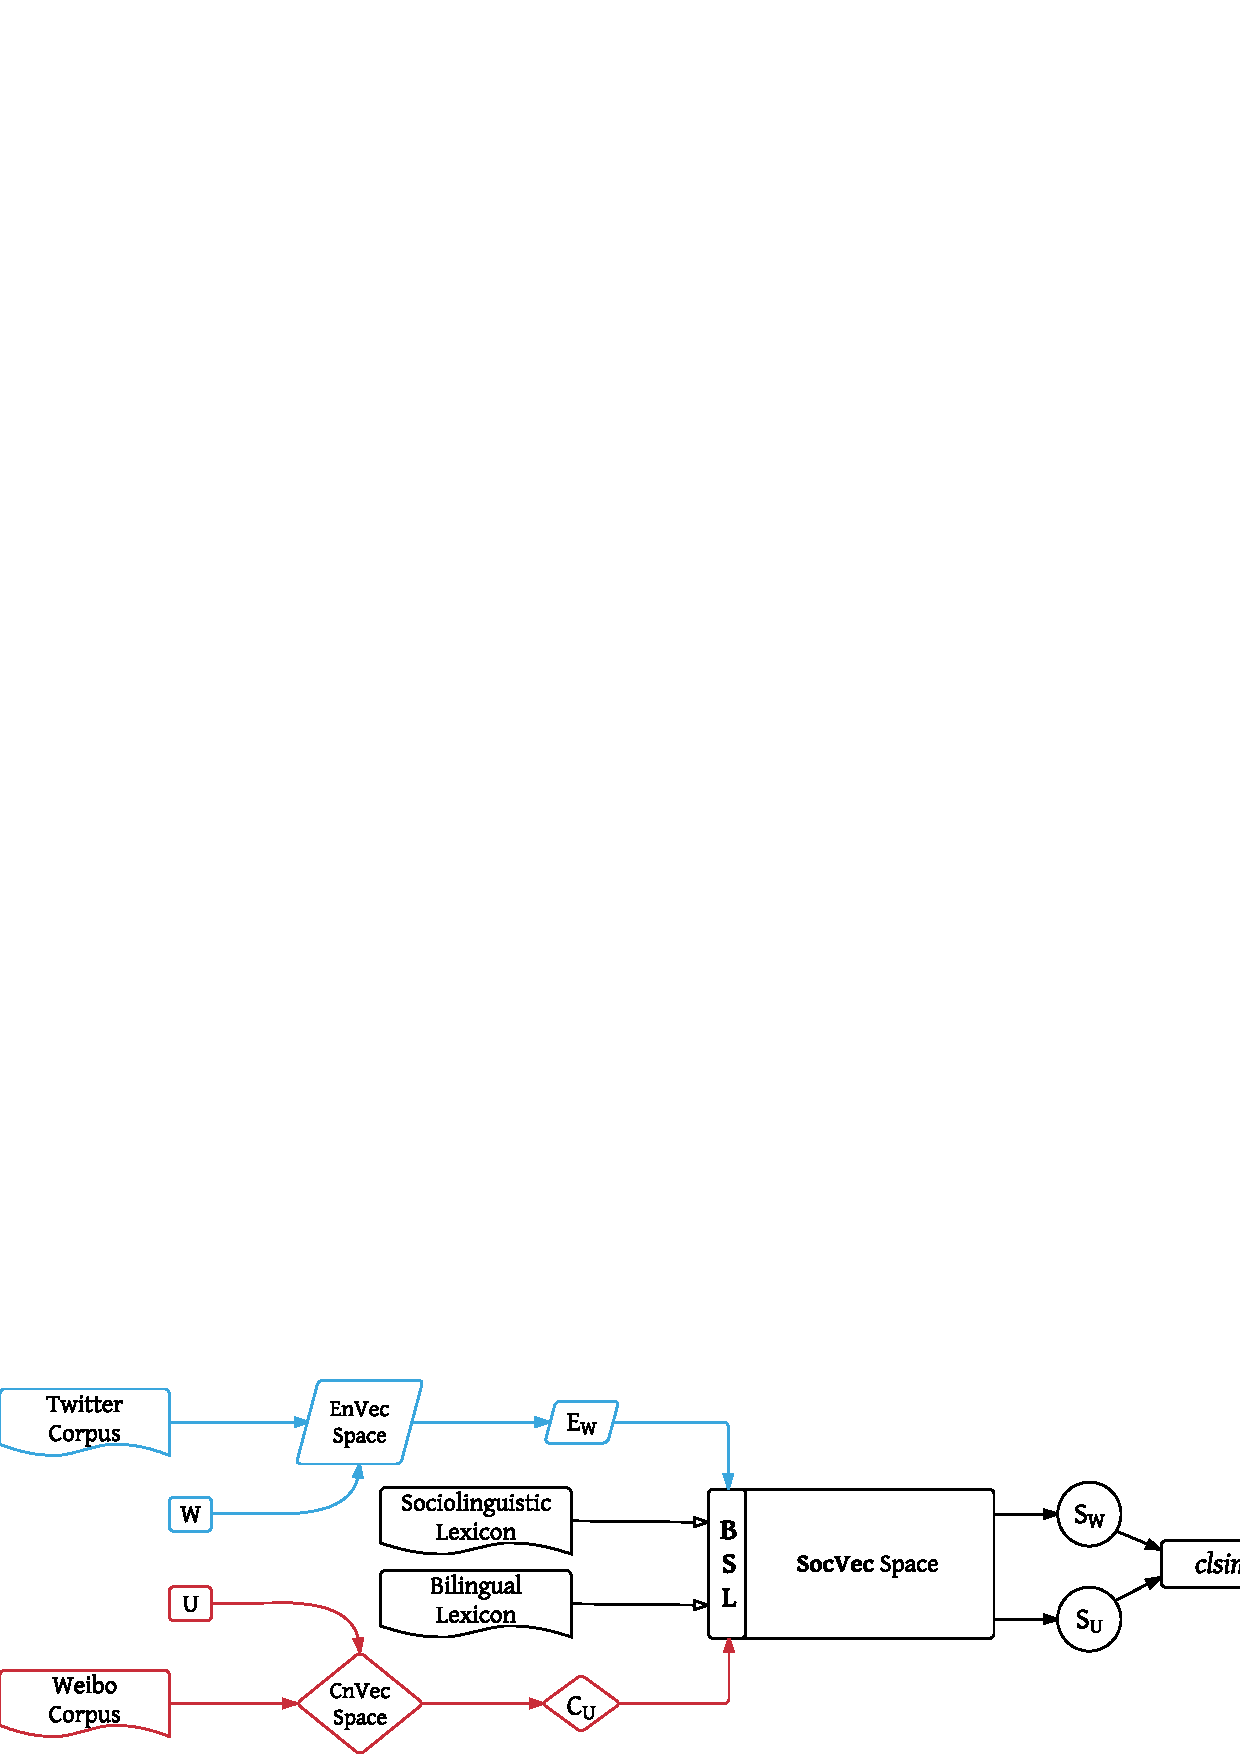
\includegraphics{figures/overview.pdf}}
	\caption{Overview of proposed neural network based joint model.}
	\label{fig:overview}
\end{figure*}


\subsection{Experimental Setup}
\label{sec:preprocess}
In this paper, we use Probase\cite{WuLWZ12} and WordNet\cite{wordnet}
as two alternative isA taxonomies. Probase is a large collection of
concept-subconcept or concept-entity pairs which were
extracted automatically by the Hearst pattern\cite{Hearst92} from
a large web corpus. Because this knowledge base is harnessed from large
data, it contains statistical scores of the extracted pairs,
such as the popularity,
and the conditional probability between the concept and its sub-concept.
WordNet, on the other hand, is a smaller, cleaner knowledge base manually
curated by experts and does not contain any scoring information.
These two taxonomies provide two different vocabularies of concepts
from which to draw the solution of AC.
%Our primary target of verb is a set of 200 most frequently used verbs in
%English text\footnote{We compute the frequency of all verbs that appeared
%in a very large web text corpus to obtain the 200 most frequently used
%verbs. We excluded a few verbs such as ``use'', ``make'', ``get'' and
%``take'' from the top of the list because they are extremely general and
%have too many arguments.},
%which we call Verb-200. These verbs are shown in \figref{fig:verbs}. A random
%sample of 20 verbs from Verb-200 forms a smaller set of verbs called Verb-20
%(highlighted in \figref{fig:verbs}) which are used in most of our experiments.

All our experiments are based on two large
datasets\footnote{We release most of
our datasets and the action concept lexicon at
\url{http://adapt.seiee.sjtu.edu.cn/~kzhu/ac}.}
from Web sentences (called Web for short) and
Google syntactic N-gram data\cite{goldberg2013,googlengram}
(called Google for short), respectively.
The 3734 most frequently used verbs (including verb phrases)
in the Web data form a primary verb set called {\bf Verb-3734}.
A subset of 2323 verbs that can be found in the Google dataset
form another verb set called {\bf Verb-2323}.
%We compute the frequency of all verbs that appeared
%in a very large web text corpus to obtain the 3734 most frequently used
%verbs.
A random sample of 20 verbs from the 200 most frequently
used verbs form the smallest set of verbs called {\bf Verb-20}
(in \figref{fig:verb20}), %which are used in most of our experiments.
which are used in some of the experiments.

The Web dataset contains 49,911,718 verb-subject pairs
and 65,035,827 verb-object pairs extracted from 165,758,215 English
sentences, which is a crawled snapshot of web pages.
%\KZ{How many subject-verb pairs and verb-object pairs in web data?}
%\KZ{How many?}\textcolor{red}{[KQ:We don't know...]}
%in a snapshot of Bing's search log.
The Google dataset contains
32,731,395 verb-subject pairs and 43,580,062 verb-object pairs
from the \emph{Verbargs} package, which includes 130,436,458
syntactic N-grams.% with verb-argument dependencies.
%\KZ{How many subject-verb pairs and verb-object pairs in google data?}
%\KZ{Kaiqi: We need to describe how we generate the web and
%google data sets here.
%Need to emphasize how big these data sets. Remember this ``VL''DB!}

\begin{figure}[th]
\centering
\fbox{\parbox{.8\columnwidth}{
bring,
carry,
connect,
cut,
define,
eat,
help,
hit,
keep,
operate,
perform,
play,
read,
release,
report,
select,
spend,
submit,
visit,
wear
}}
\caption{Verbs in Verb-20}
\label{fig:verb20}
\end{figure}

ReVerb also provides millions of relation triples, some of which contain
verbs as predicate.
%However, the scale of ReVerb is small to our problem.
We aim at discovering the action concepts,
which needs a large number of action instances
for each verb. However, ReVerb contains small number of triples for each verb.
For example, only 374 unique triples for ``wear'' are
extracted in ReVerb while our web dataset contains 17,749 unique
\pair{verb}{object} pairs for ``wear''.
The reason of the huge different is that,
a triple must contain two arguments for the verb in ReVerb. However,
verbs co-occur with only one argument in many cases.
Moreover, ReVerb has little coverage on
intransitive verbs, which only come with subject.
We give up using ReVerb data due to these limitations.
%\KZ{We need to explain why we don't use the ReVerb data.}

%\subsection{Preprocessing of Dataset}
%To make use of the web sentences and Google syntactic N-gram,
Next, we preprocess the two datasets as follows to
generate action instances.

{\bf Web} data comes from the result of Stanford dependency parser,
%We run a dependency parser on the whole corpus and
which are dependency trees for the sentences. We are interested in
verb-subject and verb-object relations only.
The head word of subject is usually labeled
as ``nsubj'' or ``agent'' while the head word of object is usually
labeled as ``dobj'' or ``nsubjpass''.
We can retrieve the entire phrase of subject or object in the dependency
tree by returning the whole subtree rooted on the head.
However, the whole phrase of subject/object is not always
a term recognizable by the taxonomies. As shown in \figref{fig:pterm},
the phrase ``a flashy baseball cap''
is extracted as the object of ``wear'', but 
it is not a valid Probase/WordNet term.
To make use of the taxonomies, we need to
detect the Probase/WordNet term from the subject/object phrase
(e.g., baseball cap).

\begin{figure}[th]
\centering
\epsfig{file=pterm.eps,width=0.8\columnwidth}
\caption{Dependency Parse Tree}
\label{fig:pterm}
\end{figure}

We use a sliding window strategy to extract longest
Probase/WordNet term that we can detect in the whole phrase.
The window slides around the head word
from right to left, and check if a Probase/WordNet term exists.
The initial size of the window is the length of the
whole phrase. If we detect a Probase/WordNet term,
we return the phrase captured in the window;
Otherwise, we decrease the window size and slides
around the head term again. We stop until we find
any Probase/WordNet term. Usually, this procedure can detect
a Probase/WordNet term from the phrase, because Probase/WordNet includes
most of the words (phrase with length 1). After
preprocessing, we output all the pairs of verb-subject and
verb-object as action instances.
%\begin{table}[th]
%\centering
%%\scriptsize
%\caption{Snapshot of Google Syntactic N-gram}
%\begin{tabular}{|l|l|}
%\hline
%Verb & N-gram \\
%\hline \hline
%accept & firms/NNS/nsubj/2\; accept/VBP/conj/0\; \\
%& money/NN/dobj/2\; in/IN/prep/2\; \\
%& exchange/NN/pobj/4   \\
%\hline
%delay & to/TO/aux/2\; delay/VB/xcomp/0\; \\
%& these/DT/det/4\; matters/NNS/dobj/2 \\
%\hline
%spent & an/DT/det/2\; afternoon/NN/nsubjpass/4\; \\
%& was/VBD/aux/4\; spent/VBN/conj/0\\
%\hline
%\end{tabular}
%\label{tab:ngram}
%\end{table}

\textbf{Google} data contains relations between
verbs and arguments.
%A snapshot
%of Google syntactic n-gram is shown in \tabref{tab:ngram}.
%The syntactic n-gram consist of the dependency parsing
%result conducted by Stanford parser.
Each token is labeled with POS tag, dependency and head index.
To apply this data to our task,
we restore each n-gram to a dependency tree according
to the head index and 
adopt the same processing as in Web to extract 
pairs of \pair{verb}{subject} and \pair{verb}{object}.
%First, we restore each n-gram to a dependency tree
%according to the head index. Next, we find the head of the
%subject or object from the nodes that directly connects to
%the verb node with a dependency label such as ``nsubj'', ``agent'', ``dobj''
%or ``nsubjpass''. Around the head, we use the same sliding window
%algorithm to find a longest Probase/WordNet term to be the subject/object
%as in the processing of the web data. Also, we convert
%the verb to its lemma form.
%After this process, we finally get two lists of pairs
%in the form of \pair{verb}{subject} and \pair{verb}{object}, respectively.

The subsequent experiments are conducted on lexicons learned from
different combinations of verb sets, taxonomies and datasets. For
readers' convenience, the configurations of these experiments are documented
in \tabref{tab:comb}.
\begin{table}[th]
\centering
%\scriptsize
\caption{Verbs, taxonomies and datasets for each experiment}
\begin{tabular}{|l|c|c|c|}
\hline
Experiment & Verb Sets & Taxonomies & Datasets \\
\hline \hline
Accuracy \& Overlap & Verb-20 & Probase &  Web, Google\\
\hline
\multirow{2}{*}{Execution Times} & Verb-3734, & Probase,
	& \multirow{2}{*}{Web, Google} \\
	& Verb-2323 & WordNet & \\
\hline
Verb Sense Matching & Verb-3734 & WordNet & Web \\
\hline
Argument Identification & Verb-20 & Probase & Web \\
\hline
WSD & Verb-3734 & WordNet & Web \\
\hline
Verb Frame Generation & Verb-3734 & Probase & Web \\
\hline
Term Similarity & Verb-3734 & Probase & Web \\
\hline
\end{tabular}
\label{tab:comb}
\end{table}

%\begin{figure}[th]
%\centering
%\fbox{\parbox{2\columnwidth}{
%\sout{use
%make
%include
%take
%get
%provide
%show}
%go
%say
%find
%see
%come
%work
%need
%look
%require
%give
%{\bf help}
%offer
%know
%create
%change
%add
%start
%allow
%{\bf keep}
%{\bf play}
%contain
%run
%apply
%receive
%call
%develop
%leave
%begin
%hold
%support
%cause
%build
%meet
%increase
%cover
%base
%want
%serve
%continue
%{\bf read}
%write
%produce
%{\bf bring}
%involve
%pay
%live
%ask
%put
%consider
%set
%reduce
%remove
%improve
%appear
%{\bf perform}
%seem
%move
%lead
%follow
%buy
%occur
%try
%design
%contact
%complete
%sell
%learn
%determine
%think
%{\bf report}
%describe
%like
%present
%mean
%relate
%lose
%feel
%affect
%post
%represent
%enjoy
%send
%open
%discuss
%{\bf visit}
%enter
%grow
%share
%maintain
%identify
%indicate
%tell
%place
%list
%return
%choose
%{\bf select}
%turn
%sign-up
%form
%obtain
%stop
%check
%result
%win
%happen
%install
%{\bf wear}
%die
%love
%understand
%save
%expect
%focus
%fill
%watch
%prevent
%{\bf spend}
%protect
%reach
%pass
%raise
%display
%treat
%ensure
%{\bf connect}
%achieve
%establish
%suggest
%view
%accept
%associate
%fit
%drive
%exist
%control
%talk
%replace
%deliver
%avoid
%hear
%fall
%let
%{\bf define}
%handle
%{\bf eat}
%plan
%bear
%prepare
%manage
%{\bf release}
%promote
%attend
%experience
%join
%kill
%seek
%{\bf operate}
%measure
%end
%refer
%teach
%face
%conduct
%explain
%purchase
%combine
%test
%{\bf cut}
%generate
%review
%deal
%break
%close
%reflect
%decide
%believe
%consist
%{\bf carry}
%fail
%collect
%speak
%address
%encourage
%match
%stand
%sit
%stay
%{\bf hit}
%{\bf submit}
%draw
%walk
%depend
%limit
%please
%reveal
%introduce
%wait
%arrive
%enable
%}}
%\caption{Verb-200 (Ranked) with Verb-20 in Bold}
%\label{fig:verbs}
%\end{figure}

%bring\\
%carry\\
%connect\\
%cut\\
%define\\
%eat\\
%help\\
%hit\\
%keep\\
%operate\\
%perform\\
%play\\
%read\\
%release\\
%report\\
%select\\
%spend\\
%submit\\
%visit\\
%wear\\
%\hline
%\end{tabular}
%\label{tab:verbs}
%\end{table}
%




\section{Framework}
%\BF{workflow figure to show the framework}
%\begin{multicols}{2}
%\begin{figure*}
%\centering
%\includegraphics[width=2\columnwidth]{sysoverviewgrapheps.eps}
%\caption{Framework wrokflow} \label{fig:workflow}
%\end{figure*}
%\end{multicols}
%\KZ{In the framework, say ``Output Parse'' instead of ``Output File.''}
The general architecture of the our parser is shown in \figref{fig:workflow}
and is divided into training phase and parsing phase.
%We take training treebank as input, which carries the
%essential information (we only use FORM and POSTAG) and
%gold dependency parses.

\begin{figure}[th]
\centering
\epsfig{file=sysoverviewgrapheps.eps, width=\columnwidth}
\caption{Sequence Based Parser Framework}
\label{fig:workflow}
\end{figure}

{\bf Training:} The preprocessing step generates oracle sequences
from the gold standard parse trees. Only the word forms and the POS tags 
in these parse trees are used. Here, we assume that a child node is
easier to process than its parent node and it is supposed to be attached
before its parent. \footnote{By this rule, multiple gold sequences
can be generated from one dependency tree. In this paper, when a parent node
has multiple children, we generate the sequence by a left-to-right order.}
%\KZ{Which one do we use or do we use all of them?}
%\footnote{
%For example, a bottom-up, breadth-first traversal of the gold parse tree or oracle transition
%process order from Malt Parser are both gold sequences.}
%and further discussion is deferred to Section 4.
%\TJ{maybe they will ask which one is the best; needs some explanations here}
We then train respectively a graph-based head mapper (a.k.a. decoder)
from the gold sequences and the gold parses, and a sequence predictor
from the gold sequences.

{\bf Parsing:} Given an input sentence, the sequence predictor
outputs a feasible decoding sequence, which is a permutation of
the words in the input. For each word in this sequence,
the head mapper returns its best head word according to a scoring function
while employing a cycle detection mechanism.
The process continues until all words in the sentence have found their
heads.
%(except manually introduce ROOT node in dependency parsing).
%For a sentence with $N$ words, the final result consists of ($N+1$) nodes
%and constructed $N$ arcs.
The procedure guarantees to produce a tree structure eventually.
\cut{
We implemented a simple version of this framework,
%and released the source code as well as the evaluation data\footnote{\urlstyle{same}\url{https://github.com/littlebeanfang/BeanParser}}.
%To reproduce the experiments refered in this paper, all our data and related commands are offered in the compressed file.
%\BF{add the data download source}
%\KZ{Besides the open-source system, create an online demo using default model
%and allow users to type in
%a sentence to have it parsed.}
and built an online demo\footnote{\urlstyle{same}\url{http://202.120.38.146/BeanParser}} to show parses of eight languages with the model
trained in our experiment.}

In the current implementation, we generate the decoding sequence by
{\em stackproj} algorithm~\cite{nivre2009non} in
malt parser and scorer-based greedy head mapper.
%\KZ{Consider rephrase this sentence.
%What does graph-based head mapper have to do with sequence?}
%The training and testing data are both in
%CoNLL format~\footnote{http://ilk.uvt.nl/conll/}.



%
% File emnlp14-rumor\paper.tex
%
\documentclass[10pt,final,conference,letterpaper]{IEEEtran}
\usepackage{times}
\usepackage{url}
\usepackage{latexsym}
\usepackage{amsmath,algorithm,algpseudocode,caption,subcaption}
\usepackage{epsfig}
\usepackage{graphicx}
\usepackage{booktabs}
\usepackage{color}
\DeclareCaptionType{copyrightbox}
%\setlength\titlebox{6.5cm}    % Expanding the titlebox
\newcommand{\triple}[3]{$\langle$#1, #2, #3$\rangle$}
\newcommand{\pair}[2]{$\langle$#1, #2$\rangle$}
\newcommand{\figref}[1]{Figure \ref{#1}}
\newcommand{\tabref}[1]{Table \ref{#1}}
\newcommand{\secref}[1]{Section \ref{#1}}
%\newcommand{\eqref}[1]{Eq. (\ref{#1})}
\newcommand{\KZ}[1]{\textcolor{blue}{[Kenny: #1]}}
\newcommand{\WK}[1]{\textcolor{red}{[Ke: #1]}}
\newcommand{\ZY}[1]{\textcolor{red}{[Zhiyi: #1]}}

\begin{document}
\title{ExtRA: Automatic Extraction of Review Aspects 
%\Thanks{}
}

\author{
Shi Feng, Kenny Q. Zhu, Zhiyi Luo\\
%Shi Feng$~^{1}$, Kenny Q. Zhu$~^{2}$, Zhiyi Luo$~^{3}$\\
%\vspace{1.6mm}
\fontsize{10}{10}\selectfont\itshape
%Department of Computer Science \& Engineering\\
Shanghai Jiao Tong University, Shanghai, China\\
\vspace{-1cm}
%\fontsize{9}{9}\selectfont\ttfamily\upshape
%$~^{1}$sjtufs@gmail.com, $~^{2}$kzhu@cs.sjtu.edu.cn, 
%$~^{3}$jessieluo1991@gmail.com
}

%\date{\today}
\maketitle
\begin{abstract}
Summarizing users opinions about a product or
service by rating against several distinct and representative aspects
is intuitive and effective. Manual determination of aspects of a product type 
doesn't scale to large and comprehensive e-commerce or consumer review sites
and doesn't adapt to changes in interests.
This paper demonstrates a unsupervised multistage
approach for automatically discovering the best aspect words from massive
amount of textual user reviews of any type of product or service. 
Our experiments showed that the approach is efficient and achieves 
the state-of-the-art accuracies.
\end{abstract}

\section{Introduction}
\label{sec:intro}

Product reviewing is a key character that distinguishes e-commerce 
from conventional retail.
Many websites provides either qualitative or quantitative
summaries of user reviews, organized by important aspects 
of the target product or service.
One example of such \emph{aspect-based review 
summarization}~\cite{hu2004mining} for a hotel on TripAdvisor
as of June 2016 is shown in \figref{fig:tripadvisor}. 
Here, besides the short review passage written by the user, 
the user are asked to give discrete ratings (on the scale of 1-5) 
on various aspects of the hotel room, 
e.g., location and cleanness. The ratings of 
a product from individual reviews can then be aggregated into an overall
ratings of the same product by many users.

\begin{figure}[th]
\centering
\includegraphics[width=0.7\columnwidth]{figures/tripadvisor-short}
\caption{Part of a user review from TripAdvisor.}
\label{fig:tripadvisor}
\end{figure}


Aspect-based review summaries strike a nice middle ground between
detailed text reviews and an all-in-one overall score, yielding
a somewhat balanced view of a product. Such summaries
provide an effective and efficient way of comparing products in
the same category.
%have several advantages compared to the more traditional 
%style of online reviews that consists of a short passage and 
%an overall rating. 
%In aspect-based reviews, more details are provided quantitatively and 
%more directly, and the users can learn about various aspects of a product 
%without having to read the entire review passage. Another advantage of 
%aspect-based reviews is that different products within the same category 
%can be compared directly with respect to multiple aspects, 
%instead of just an overall rating. When researching on products, 
%users spend most of their time comparing different brands and models. 
%Aspect-based review summarization provides an effective and efficient way for 
%doing such comparison, saving the users both time and effort.


%At present, websites that offer aspect-based review summaries typically 
%only feature a single or a small number of product categories, e.g.,
%TripAdvisor.com only features travel related products while Cars.com reviews
%automobiles. 
Because it takes in-depth knowledge to 
characterize a product type using a few keywords that balance between
relevance and diversity, at present, these aspects are primarily hand picked
by the review site operators.
Manual selection of aspects cannot scale to large number of
product types as featured by general e-commerce platforms such as Amazon.com
and Yelp. Moreover, such aspects may change from time to time due to 
evolving user interests.
%These platforms instead turn to automatic review 
%summarization, mined from the user review texts. 

%\begin{figure}[th]
%\centering
%\includegraphics[width=0.8\columnwidth]{figures/phrases}
%\caption{Automatic review summarization for two mobile phones 
%on an e-commerce website}
%\label{fig:phrases}
%\end{figure}
%
%An example of automatic review summarization commonly seen 
%on e-commerce websites is shown in \figref{fig:phrases}. 
%There is a summary of opinion phrases for each phone model, 
%along with the frequency of each phrase mentioned in the 
%reviews. There are two major drawbacks in this form of summarization. 
%First, it is restricted to using the reviews about a specific product. 
%Therefore, summaries are incompatible across different products within 
%the same category - different models may not share the same set of 
%opinion phrases. This makes it less useful for users to compare
%different models.  Second, users' sentiment toward 
%each aspect cannot be quantified and computationally compared - 
%the difference of emotional strength between 
%``extremely good" and ``above average" is hard to capture.
% user cannot choose to express them differently.

%The aspects of a product are supposed to capture the most important features 
%and cover all the facets of the product. The products of the same category 
%share the same set of aspects, however the aspects can be very different 
%across categories. It takes both common knowledge and personal experience 
%with the product to decide which are the appropriate aspects. 
%The websites that can provide aspect-based rating system basically 
%all share a common feature, that is they each focuses on only one or 
%a small range of products. For example TripAdvisor focuses on hotels and 
%Cars.com focuese on cars. The set of aspects is what the consumers base 
%on to compare different products, thus they must be carefully chosen 
%to cover all the facest of the product. Moreoever, at the end of the day 
%the aspects is designed to serve the consumers, especially potential consumers, 
%so they need to reflect what the consumers care about the product. 
%Ideally, the aspects should be decided with user reviews taken into 
%consideration. For a small range of products, the website owner or 
%the retailer may manual designate the set of aspects, 
%however this is intractable for websites like Amazon and TaoBao, 
%which host basically all kinds of products available on the market, 
%and websites like Yelp on which users review thousands of different services. 
%
%Motivated by this observation, we are in need for methods that automatically 
%generate review summarizations. 

Our goal in this paper is to develop an unsupervised system 
for aspect word extraction from a set of user reviews about products within 
the same category.  This problem is similar to topic modeling where aspects 
can be seen as topics, but with a few differences: 
\begin{itemize}
    \item in aspect extraction, we seek to produce 
	aspect words with small mutual semantic overlap; 
    \item aspects may be expressed implicitly through personal experience; and
    \item reviews are a short piece of text, 
	  hence the topics may shift very quickly from 
          sentence to sentence.
\end{itemize}
Previous unsupervised methods for aspect extraction are 
variations of topic models, and cannot capture word semantics and thus
the implicit reference of product aspects. 
In our method we leverage the distributed 
representations of words and sentences. With distributed representations, 
the semantic similarity between two sentences can be more accurately 
calculated without relying too much on the lexical information.
Our proposed method consists 3 clustering steps and
2 ranking phases. The framework achieved state-of-the-art performance 
in end-to-end aspect extraction across multiple domains.

%In \secref{sec:method} we introduce our method step-by-step.
%In \secref{sec:experiments} 
%we evaluate our method on user reviews from multiple domains and demonstrate 
%the effectiveness of our model against other approaches 
%and show how the aspects extracted can be used
%to construct a complete review summarization. 
%In \secref{sec:related}, we discussed
%and compare our work with previous research on aspect-based review 
%summarization.

\section{The System}
\label{sec:method}

The review aspect extraction problem aims to infer $K$ noun 
words from user reviews about the same product type.
Each word represents a distinct aspect or feature of the product type. 
%Here $K$ is an constant parameter for the problem. 
%In unsupervised models for aspect extraction, 
%the set of reviews and the number of aspects are the only inputs.
%Note that in this definition we don't use cross-domain information, 
%that is, for one product type we only use the reviews of that domain.
%This allows us to apply the model to any domain with ease.
%\begin{figure}[th]
%\centering
%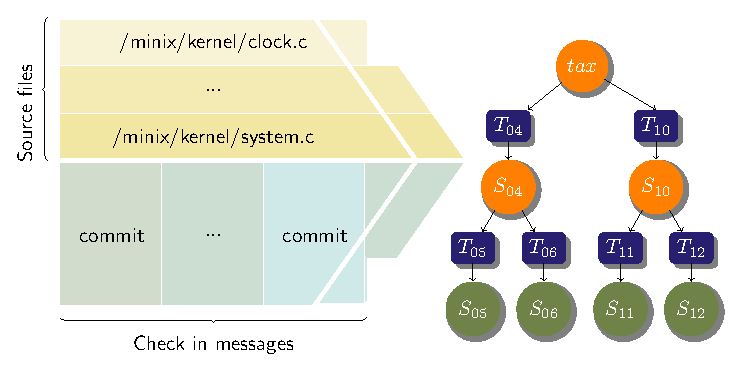
\includegraphics[width=0.9\columnwidth]{figures/framework}
%\caption{Our framework.}
%\label{fig:framework}
%\end{figure}
%
Our system framework consists of 5 steps.
%
%\begin{itemize}
%    \item \textbf{Sentence Clustering}
%
%        We convert each sentence in the reviews into a vector representation 
%        and cluster them in to $N$ clusters of semantically similar sentences.
%
%    \item \textbf{Noise Isolation}
%
%        %As aspects appear as topics in the reviews, 
%        %we use a topic model to infer the potential aspects.
%        To isolate the noises that exist in the sentence cluster,
%	for each sentence cluster we further generate $M$ 
%	topics, resulting in $N\times M$ different word distributions in total.
%
%    \item \textbf{Aspect Inference}
%        
%        We treat each word distribution as a vector and cluster the topics 
%	into $C$ clusters which are the potential aspects. 
%	Here $C$ is purposely set to be larger than $K$. The extra
%	$C-K$ clusters models the redundant aspects.
%        Each cluster contains $N\times M / C$ word distributions, or vectors.
%        We take the mean of these vectors to form $C$ aspect clusters,
%        each being a set of words and their corresponding weights.
%
%    \item \textbf{Cluster Ranking}
%
%        We define a score for the quality of each aspect cluster,
%        and the clusters are ranked by this score.
%
%    \item \textbf{Word Ranking}
%
%        We use WordNet to calculate the semantic distances between the words 
%	in each cluster and adjust the ranking based on the 
%	both the distances and the weights of the words. The top words in each
%	cluster are candidates of the aspect words.
%\end{itemize}
%
%In the following we will explain the motivation and the details of each of
%the five steps. 
%
\subsection{Sentence Clustering}

%One important feature of user reviews is that many topics are 
%compressed into a short paragraph, where each topic corresponds to 
%a potential aspect of the product. 
%A typical hotel review extracted from \figref{fig:tripadvisor} 
%is shown as follows:
%
%\begin{quote}
%Pool is small and only 4 ft but refreshing. Hot tub also there. Staff were super friendly each day. Room was nothing special but clean and comfy. Lots of restaurants and bars nearby. Breakfast was great and despite being a busy weekend there was always a big selection available.
%\end{quote}
%
%In user reviews, topics can shift very quickly.
%Sentences that are close to each other may refer to 
%completely different aspects about the product. Also,
%sentences about the same aspect may not appear in the review consecutively. 
%The existence of such fine-grained semantic shifts in user reviews 
%makes it difficult to apply the the bag-of-word abstraction 
%of normal topic model on reviews.
%Therefore we propose to work on the sentence level instead 
%of the document level, and it would be helpful if we can divide the 
%reviews into topic-oriented segments.
%
%Driven by this observation, in our method the first step is 
%sentence clustering.  For this purpose, 
We represent each sentence in a high-dimensional vector space,
%Instead of using simplistic methods like bag-of-word vector, 
%we leverage a recent development of neural network in natural 
%language processing, the distributed representation.
%In a distributed representation, words and sentences are 
%converted into real-valued vectors.
%The distance of the vectors in the vector space will capture the 
%semantic similarity of the words or sentences.
%In this work we attempt two models, 
using either LSTM (a variant of RNN) or paragraph vector (PV) \cite{le2014distributed}.
%
%\paragraph{Recurrent Neural Network}
%To use RNN for obtaining sentence vectors, 
%we train a neural language model on the review sentences. 
%After the perplexity converges, we use the trained network to 
%process each sentence of the dataset and take the last hidden vector as 
%the vector representation of the sentence. In our method we use a 
%variation of RNN, long-short term memory (LSTM)~\cite{hochreiter1997long} 
%which is reported to have better performance at 
%modeling long sentences \cite{jozefowicz2015empirical}.
%
%\paragraph{Paragraph Vector}
%PV is a simple but powerful extension to Word2vec \cite{mikolov2013distributed} with two components, 
%distributed memory (PV-DM) and distributed bag-of-word (PV-DBOW). 
%The first one is similar to skip-gram in Word2vec and 
%the second is similar to CBOW \cite{mikolov2013distributed}.
%An important advantage of paragraph vector models is that they require 
%no labeled data. Also, it doesn't require human experts to assign weights 
%for words in a paragraph based on linguistic knowledge. 
%The learned vector representations inherit an important property of Word2vec, 
%that is the semantics similarity. Also the final paragraph vector captures the 
%word order information with the part learned from PV-DBOW with the n-gram model.
An advantage of paragraph vector over RNNs is that it can 
leverage trained word vectors, thus requires a smaller training data set. 
%The word vectors can be trained on 
%a much larger corpus so they capture the semantics relationships more 
%accurately.  Consequently, the paragraph vectors can be trained on 
%a relatively small dataset. 
%The performance of paragraph vectors can also be boosted by using pre-trained 
%word vectors that are trained on a larger dataset \cite{mikolov2013linguistic}. 
%%However, previous research show that it is more suitable 
%%to train the word vectors simultaneously for RNNs, 
%%so RNNs cannot leverage the word vectors learned from a larger dataset. 
%Also, the paragraph vector models are simple and 
%don't require the storage of a lot of information. In contrast, for RNN we 
%need to store every state during the forward pass for back-propagation, 
%which is very memory consuming.
%\paragraph{Clustering Sentence Vectors}
We run k-means clustering on the sentence vectors and generate 
$N$ sentence clusters. We then collect the sentences from the same review 
that are clustered together to form smaller fragments of reviews. 
Each original review is divided into several smaller review fragments, 
each belonging to one of the $N$ clusters. As a result, we obtain $N$ 
clusters of review fragments. 

\subsection{Noise Isolation}
There exists noises and overlaps in the clusters formed above.
%The first step, sentence clustering, we might include noise and the sentences 
%within a cluster might not all be about the same aspect. 
%The reason is due to the common occurrences of sentences such as the following
%in the reviews (taken from TripAdvisor):
%
%\begin{quote}
%The room was clean, the staff were friendly, and I would say the price is very reasonable given the proximity to business and leisure destinations around downtown.
%\end{quote}
%
%\begin{quote}
%There is a restaurant just 5 min walk away with nice italian food, pizza was great.
%\end{quote}
%
%In the first sentence multiple aspects are mentioned; in the second sentence, the only aspect is location however lexically it seems to be talking about food.
%With these complicated structures within, 
%it is difficult for RNN or PV to correctly determine the aspects 
%in these sentences. The result is overlaps between clusters about 
%different aspects and noises within each cluster.
%To isolate the noises and resolve such overlap, 
We fix that by applying LDA topic modeling within each sentence cluster, 
treating each review fragment as a document, and generating $M$ smaller topics. 
This will give us in total $N\times M$ topics, or, word distributions. 
%\tabref{table:overlap} shows an example of topics inferred from three
%sentence clusters from hotel reviews and illustrates the overlap problem.
%In this example, five topics were extracted from each sentence cluster, 
%and each row is one topic. It can be seen that the aspects for the 
%three clusters should be {\em room}, {\em location} and {\em price} 
%respectively.
%However, topics shown in boldface font obviously belong to 
%other clusters.  Especially, the last topic of the third cluster 
%appears to be an overlap of more than two clusters.
%The noise isolation step effectively separates the noise topics from other
%topics semantically corehent within a sentence cluster.
%
%\begin{table}[th]
%\centering
%\caption{Topics extracted from three sentence clusters of hotel review.}
%\label{table:overlap}
%\begin{tabular}{|c|l|}
%\hline
%& room bed bedroom size floor \\
%Sentence
%& bedroom room wall size decor \\
%cluster 1
%& room bathroom shower water towel \\
%& room suite size view floor \\
%& room shower area kitchen bed \\\hline
%
%& station minute tube location bus \\
%Sentence
%& location price night place rate\\
%cluster 2
%& location square station street subway\\
%& distance bus subway downtown shopping\\
%& \textbf{restaurant} \textbf{city} \textbf{food} \textbf{buffet} \textbf{place} \\\hline
%
%& price rate service money star\\
%Sentence
%& \textbf{location} \textbf{city} \textbf{star} \textbf{time} \textbf{rate} \\
%cluster 3
%& price service night money city\\
%& price location place night city\\
%& \textbf{location} \textbf{service} \textbf{food} \textbf{price} \textbf{restaurant} \\\hline
%\end{tabular}
%\end{table}


\subsection{Aspect Inference}
\label{sec:topic_clustering}
Each topic is a word distribution, represented by a vector. 
We obtain  more compact representations of those topics by using PCA to 
reduce the topic vectors to 100-dimension.
%We use PCA to reduce the topics vectors to 100-dimension by  
%selecting the 100 words that best distinguish different topics.
Then we perform k-means clustering on the $N\times M$ topics vectors to 
generate $C$ clusters, each containing $(N\times M)/C$ topics.
These are called {\em aspect clusters}.
We set $C$ to be slightly larger than the desired number of product 
aspects $K$, so that the noisy topics can be clustered together and 
later discarded. 
%In an experiment we will evaluate the influence of this redundant clusters on 
%the quality of the final aspects.
%
%\begin{table}[th]
%\caption{Aspect clusters extracted from hotel reviews.
%Each row shows the candidate words of an aspect, sorted by the weight of each word.}
%\label{table:step3}
%\centering
%\begin{tabular}{|l|} \hline
%breakfast, meal, food, tasty, dinner, morning, coffee, tea \\\hline
%room, night, time, bed, day, bathroom, staff, area, place \\\hline
%staff, desk, service, friendly, reception, concierge, helpful \\\hline
%close, city, location, place, central, station, bus, street\\\hline
%bed, shower, spacious, room, size, bathroom, bedroom, floor \\\hline
%price, room, check, night, money, city, location, star, service \\\hline
%location, price, room, night, place, rate, money, time, city  \\\hline
%\end{tabular}
%\end{table}
%
%Finally, for each cluster we take the mean of the $(N\times M)/C$ 
%topics and normalize it
%for the word distribution of that cluster.
%Some example aspect clusters extracted from hotel reviews are 
%shown in \tabref{table:step3}.

\subsection{Cluster Ranking}

We rank the clusters by how ``distinct'' each cluster is from other clusters. 
If a cluster is similar to other clusters, it is considered redundant and of
low quality. We discard $C-K$ least distinct clusters.


%For the $i$th cluster $C_i$ ($i\in [1, C]$), 
%the distinctiveness score $S(i)$ is defined by:
%
%\begin{align}
%S(i) &= \sum_{w\in C_i} S_i(w) \nonumber\\ 
%     &= \sum_{w\in C_i} \log\left(\frac{f_i(w)}{\sum_{j\neq i} f_j(w)}\right)\nonumber \\
%     &= \sum_{w\in C_i}\left[\log f_i(w) - \log\sum_{j\neq c} f_j(a)\right]
%\end{align}
%
%\begin{table}[t]
%\caption{Aspect clusters ranked by distinctiveness score.
%Potential aspect words are boldfaced.}
%\label{table:clustersranked}
%\centering
%\begin{tabular}{|l|} \hline
%\textbf{staff}, desk, \textbf{service}, friendly, reception, concierge, helpful \\\hline
%breakfast, meal, \textbf{food}, tasty, dinner, morning, coffee, tea \\\hline
%\textbf{price}, room, check, night, money, city, location, star, service \\\hline
%bed, shower, spacious, \textbf{room}, size, bathroom, bedroom, floor \\\hline
%close, city, \textbf{location}, place, central, station, bus, street \\\hline
%\textcolor{red}{room, night, time, bed, day, bathroom, staff, area, place} \\\hline
%\textcolor{red}{location, price, room, night, place, rate, money, time, city} \\\hline
%\end{tabular}
%\end{table}
%
\subsection{Word Ranking}
\label{sec:word_ranking}

We rank the words in each cluster 
by considering two factors (similar to TF-IDF): 
the representativeness of the word to the host
cluster; the number of times the word appears in other clusters. 
The most representative word in each cluster
is assumed to be the closest to the centroid of the word cluster.
The distance between two words is the inverse of 
cosine similarity between the word2vec
vectors of the two words.
Then we process the clusters in the order of 
the cluster ranking given in the last step.
When we calculate the score for word $x$ cluster $C_i$,
we also consider the scores of word $x$ in clusters $C_1$ to $C_{i-1}$, 
where the scores have already been calculated. 
We prevent the duplicate aspect words by subtracting the scores 
of $C_1$ to $C_{i-1}$, from the score of $C_i$.
%The score of word $x$ in the $i$th cluster $C_i$ is thus defined by:
%
%\begin{equation}
%s_i(x) = u_i(x) \sum_{y\in C_i}\hat{x}\cdot \hat{y} - \sum_{j=1}^{i-1}s_j(x),
%\label{eq:wordscore}
%\end{equation}
%where $\hat{x}$ is the vector representation of x; $u_i(x)$ is the weight of $x$ in cluster $C_i$.
The words in each cluster is thus ranked by this final score.

\section{Evaluation}
\label{sec:experiments}

We evaluated our framework
against a number of baselines including the state-of-the-art approaches.
%in the end-to-end aspect extraction task.
Our dataset is reviews for 15 categories of product or service crawled from
e-commerce sites such as Amazon.com and Yelp. 
%The review content is plain English text and we do not use any labels 
%for training our model. We use human labels for evaluation. 
%The product categories, their sources and the sizes of the review datasets
%are summarized in \tabref{table:dataset}
%
%\begin{table}[th]
%\centering
%\caption{Dataset summary.} 
%\label{table:dataset}
%\begin{tabular}{|c|c|r|r|}
%\hline
%Product type & Source & No. of Reviews & No. of Words \\ \hline \hline
%hotel        & TripAdvisor & 27145   & 210 \\\hline
%mobile phone & Amazon & 3716    & 136 \\\hline
%mp3 player   & Amazon & 2745    & 128 \\\hline
%laptop       & Amazon & 5471    & 97  \\\hline
%tv           & Amazon & 1237    & 102 \\\hline
%shoes        & Amazon &1748    & 82  \\\hline
%headphone    & Amazon & 1647    & 122 \\\hline
%gps          & Amazon & 1726    & 72  \\\hline
%transportation & Yelp & 3077  & 131 \\\hline
%restaurant   & Yelp & 4016    & 176 \\\hline
%gym          & Yelp & 2481    & 230 \\\hline
%shopping     & Yelp & 2718    & 123 \\\hline
%car dealer   & Yelp & 2839    & 190 \\\hline 
%movie        & Pang et al. \cite{pang2002thumbs} & 3000    & 194 \\\hline
%car          & Cars.com & 1074    & 147 \\\hline
%\end{tabular}
%\end{table}
%
%
%For evaluation, we ask 5 college students proficient with English 
%to annotate ground truth
%aspect words for each product category. For each category, 
%we ask them to provide 5 different words that cover the most important 
%aspects of the corresponding product or service. The labels provided by the
%5 annotators are aggregated together without removing duplicated words, 
%so we have 25 words in total. 
%When evaluating the models, 
%we compare the 5 aspect words generated by the models with those provided 
%by the annotators. 
%We calculate the portion of words among the 25 labels that 
%are correctly generated by the model as the accuracy of the model.
%The ground-truth labels for two product categories are shown 
%in \tabref{table:labels}.
%
%
%\begin{table}[th]
%\centering
%\caption{Labels for hotel and shopping. Each row is provided by one annotator.}
%\label{table:labels}
%\begin{tabular}{|c|l|}
%\hline
%\multirow{5}{*}{hotel}
%& room price location service utility \\
%& room service price food location  \\
%& sleep service room price location  \\
%& location price bedroom bath staff  \\
%& room price bath staff location  \\\hline
%
%\multirow{5}{*}{shopping}
%& location product service price environment \\
%& product price service location ambience \\
%& price food location size facility \\
%& sales location food service environment \\
%& price location service facility food \\\hline
%\end{tabular}
%\end{table}
%
%\subsubsection{Parameter Tuning}
We conduct a few experiments to determine the following
parameter settings: $N=10$, $M=10$, $C=K+2$, i.e. at most two extra clusters.

We compare 5 models in our experiments, 
LDA as a simple baseline, 
D-PLDA \cite{moghaddam2012design} as a representative for joint 
aspect-sentiment models, MG-LDA \cite{titov2008modeling} as 
a representative for aspect extraction topic model,
and two variations of our model LSTM and PV. 
We run the 5 models on the review data of each product type separately. 
For the main experiment, the number of aspects is fixed to 5.

%\begin{figure*}[th]
%\centering
%\includegraphics[width=1.9\columnwidth]{figures/results}
%\caption{Accuracies from different models.}
%\label{fig:results}
%\end{figure*}
%In the end-to-end evaluation, we compare the performance of our models on aspect extraction with three other models as mentioned above. The results are shown in \figref{fig:results}. 
By the accuracy, our two models out-performed all other models in 13 out of 15 
categories. The PV model performs better LSTM, 
which is consistent to our earlier analysis. \tabref{table:hotel_aspect_words}
shows the 5 aspect words by each model for hotel reviews.

\begin{table}[th]
\centering
\small
\caption{Top aspect words for hotels by different models}
\label{table:hotel_aspect_words}
\begin{tabular}{|l|l|} \hline
Ours(PV) & staff, food, price, room, location \\ \hline
Ours(LSTM) & service, location, time, food, bed\\ \hline
MG-LDA & shower, time, food, room, price\\ \hline
DP-LDA & service, station, check, coffee, bed \\ \hline
LDA & stay, location, room, staff, room \\ \hline
\end{tabular}
\end{table}
 
\section{Demo Scenarios}
We present a web demo which depicts the following scenario.
The user logs on and selects
a product type, e.g. ``cell phones'', from a predefined set of categories,  
and sets the number of aspects $K$. 
Then the user clicks the ``generate" button to extract $K$ aspect words for the selected product type.
Upon this, the system computes the review summaries of all cell phones. 
%Upon this, the system shows the $K$ precomputed aspect words for that
%product type, computed from the many user reviews about ``cell phones''. 
%Then the user clicks a button to ``generate review summaries'', which presents
%the review summaries of all cell phones in
%the system. 
Each summary contains the aspects and their scores, computed from the sum of
sentiment scores (1, 0 or -1) against each aspect using LSTM trained on
Stanford Sentiment Treebank~\cite{socher2013recursive}. 
The user may filter out some of the 
results by using the search box (see \figref{fig:summary1}). 
If the user wishes to understand why a product receives a score for a 
certain aspect, they can click on the ``xxx customer reviews'' link
and be directed to the original review snippets with the aspect words and 
sentiment words highlighted. The review snippets by can further grouped by
aspects by clicking on the tabs (see \figref{fig:summary2}). 

\begin{figure}[th]
\includegraphics[width=\columnwidth]{figures/demo1.png}
\caption{Automatically generated 6 aspects for cell phones}
\label{fig:summary1}
\end{figure}

\begin{figure}[th]
\includegraphics[width=\columnwidth]{figures/demo21.png}
\caption{Review snippets displayed by the aspects}
\label{fig:summary2}
\end{figure}


%The second and a minor scenario enables the user to examine the dynamic change
%in aspect words over time for each product type. The system shows a time line,
%annotated with different sets of aspect words, by configurable time periods,
%e.g., every month, 6 months or a year.  
 
\bibliographystyle{IEEEtran}
\bibliography{master}
\end{document}


\section{Experiments}
\label{sec:experiments}
In this section, we conduct
extensive experiments on slogan generation 
to evaluate the performance
of the proposed model SALE.
We introduce the dataset, 
the competing models and parameter settings,
as well as the evaluation metrics.
We also demonstrate the experimental results in a series of evaluations
and perform further analyses on the effectiveness of our approach
in generating accurate, fluent, informative and attractive slogans.

\subsection{Dataset}
\label{sec:dataset}
We first introduce the text corpora we create
for slogan generation task in e-commerce.
Then we describe the evaluation dataset we used in
our following experiments.
The datasets are released at \url{https://202.120.38.146/slogan/}.

\subsubsection{Dataset for Slogan Generation}
\label{sec:corpora}
%In this section, we describe the experimental setup,
%especially the hyper-parameter configurations of 
%the Seq2Seq framework we used in following experiments. 
%We also detail dataset used in our experiments.
Slogan generation in E-commerce is a relative new problem.
Thus, there is a lack of dataset for this task.
We created a new dataset, containing 
the basic information of the topics attending to potential focuses or selling-points,
including the topic and its item preference, as well as the slogan.
The data are collected from Taobao, a large-scale website for e-commerce in China.

We use the pattern of ``\emph{PV} + \emph{CG}" 
to construct topics from frequent phrases mining from largely amount
of query logs and product titles.
The product titles are composed by the sellers and content producers on the
website.
We construct multiple item preferences for each topic by sampling items from 
secondary categories as well as human intervention to 
make the items with an item preference concentrate more on a specific focus 
or selling-point.
Thus, in each instance, a topic is annotated with an item preference semi-automatically
by leveraging the category ontology introduced in \secref{sec:introduction}.
Then, we recruit experts to write a slogan for each data instance.
Overall, the dataset contains 857 topics and 
in total 3,555 $(x, p, y)$ instances after preprocessing.

We use four splits named (train/dev/LMdev/test) in our experiments.
Note that, the LMdev split is for 
hyper-parameter $\beta$ tuning (see \secref{sec:shallow_fusion} in details).
The splits are randomly divided based on topics 
proportionally by 90\%, 5\%, 1.5\% and 3.5\%.
Thus each split of (train/dev/LMdev/test) includes 771, 43, 13, 30 topics separately,
and correspond to 3132 training instances, 231 development instances, 
50 LM development instances, as well as 142 test instances.

%For the evaluation dataset, 
\subsubsection{Evaluation Dataset}
\label{sec:eval_dataset}
We perform algorithm evaluation and human evaluation
in our experiments (see \secref{sec:metrics} in details).
Thus we provide two evaluation datasets separately for each.
We directly use all the 142 instances of test split in \secref{sec:corpora},
referred as FULLtest,
for the algorithm evaluation which are based on automatic scoring systems,
such as BLEU.
Besides, we randomly sample 50 instances from the test split
to form a small evaluation dataset for human evaluation,
referred as HUMtest.


\subsection{Compared Methods}
\label{sec:compared}
In this section, we introduce the baseline and choices for 
our model components, as well as the parameter settings
used in those models.

\subsubsection{Baselines and SALE}
\label{sec:baselines}
According to the problem statement (in \secref{sec:problem})
and the proposed item preference fusion methods (in \secref{sec:preference}),
the models for comparison backed by Seq2Seq framework are mainly one-way input models and two-way input models.

One-way input models (prefixed by \emph{One}) takes in one-way input as the source sequence,
and the slogan as its target sequence, without considering 
semantics enhancement or incorporating pretrained language model.
There are three one-way input baselines with different inputs.
\textbf{One-T} (\textbf{t}opic) model
takes the topic itself as its source sequence,
while \textbf{One-P} (item \textbf{p}reference) model takes
the titles of items as its source sequence.
Then, 
%while 
\textbf{One-CAT} (con\textbf{cat}nating) model 
concatenates the topic and its item preference with special token \emph{SEP}
as a separator, and takes the sequence of concatenation as its source sequence.

The two-way input models (prefixed by \emph{Two})
are designed to treat topics and item preferences heterogeneously.
We propose two kinds of two-way input models
based on different heterogeneous inputs fusion methods 
(see details in~\secref{sec:preference}).
%we propose two fusion methods in \secref{sec:preference}
%to combine the heterogeneous inputs.
\textbf{Two-BiAttn} (\textbf{bi}directional \textbf{att}ending) model use the two-way bidirectional attending
to combine the representations of topics and that of item preferences.
\textbf{Two-CAT} (con\textbf{cat}nating) model use two-way concatenating strategy 
to fuse the heterogeneous outputs of encoders.

For \textbf{SALE}, 
we incorporate the semantics enhancement module
(in \secref{sec:semantics}) to enrich
the deep contextualized representations
backed by Two-CAT baseline.
\textbf{SALE+PLM} integrates
%On the basis of SALE, 
%we integrate
pre-trained language model (PLM) 
into SALE at inference time in order to improve
the generalization and robustness of the model.
%Specially, SALE identifies the \emph{is-a} relations
%among heterogeneous inputs and
%increase the semantic capacity of the model for better contextualized representations
%knowledge-aware module

\subsubsection{Parameter Settings}
We use an architecture of 8 stacked convolutional layers 
for both the topic encoder and the item preference encoder
as well as the decoder parts with kernel width as 3.
To enable deep convolutional networks, 
we add residual connections~\cite{he2016deep} from the input of each convolution
to the output of the layer as well.
For each convolutional layer, we set the hidden vector size as 512
and the embedding size as 256.
To alleviate the overfitting problem, we add the dropout ($p=0.2$)
layer~\cite{srivastava2014dropout} for all convolutional layers and fully connected layers.

To optimize the proposed models,
we use Nesterov's accelerated gradient method
~\cite{sutskever2013importance} with gradient clipping 0.1
~\cite{pascanu2013difficulty},
momentum 0.99, and 
learning rate 0.2.
We terminate the training process when the learning rate drops 
below 10e-5.
We set beam size as 5 for the beam search algorithm
in the testing step.
The hyper-parameter $\beta$ of SALE-PLM (in ~\eqnref{eq:shallow_fusion})
was selected to maximize the generation performance
on the LMdev split by grid search, from the range 1e-4 and 0.1.


\subsection{Evaluation Metrics}
\label{sec:metrics}
We perform both algorithm evaluation and human evaluation
in our experiments.
Specially, we evaluate our model on generation quality which includes
the automatic scoring metrics such as
BLEU and lexical diversity,
as well as a number of human-evaluation metrics.

\paragraph{BLEU}
The BLEU algorithm~\cite{papineni2002bleu} compares consecutive phrases of the 
generated slogan with the consecutive phrases it finds
in the reference slogan, and counts the number of matches, in a weighted fashion.
A higher BLEU score indicates a higher degree of similarity with the reference
slogan.
We compare all competing models on test split in terms of the BLEU score as a sanity check.
We also use BLEU score as the standard metric to finetune
hyper-parameter $\beta$ in SALE+PLM model.

\paragraph{Lexical Diversity}
A common problem in automatic text generation is that the system tends to generate safe
answers with enough diversity~\cite{li2016deep}.
A low diversity score often means generated contents are general and vague, 
while higher diversity means the generated contents are more informative and 
interesting.
Following~\cite{ChenLZYZ019}, we calculate the number of distinct n-grams produced on the test split
as the measurement of the diversity of generated descriptions.

\paragraph{Human-evaluation Metrics}
Automatic scoring metrics including BLEU score and lexical diversity are competitive and inexpensive to operate.
However, they do not consider
other important aspects such as intelligibility and grammatical correctness (or fluency) of slogan.
We use several human-evaluation metrics
to evaluate competing models on various perspectives.
\begin{itemize}
	\item \textbf{Overall quality} is designed to measure the
	overall generation quality of model.
	\item \textbf{Relevancy} is used to measure the content relevancy of generated slogan to the given topic and items.
	\item \textbf{Fluency} focus on the intelligibility and grammatical correctness of generated slogan.
	\item \textbf{Interestingness} takes personification and attractiveness into account.
\end{itemize}


\subsection{Performance Comparisons and Analysis}
\label{sec:results}


In this section, we conduct an analysis of our proposed model
to evaluate the contribution of item preference fusion module and
semantics enhancement module as well as the integration of 
pre-trained language model.

We evaluate competing models on FULLtest and HUMtest 
as we described in \secref{sec:eval_dataset}.
The comparison results of slogan generation are shown in 
\tabref{tab:auto_eval} and \tabref{tab:human_eval}.
For human evaluation, we recruit three experts as annotators 
and ask them to give scores on each aspect of generated slogan, 
range from 1 to 5,
then average the scores of each aspect on HUMtest as 
human evaluation results.


\begin{table*}[th]
	%	\small
	\centering
	\caption{Slogan generation results comparison with baseline methods using FULLtest.}
	\label{tab:auto_eval}
	\begin{tabular}{lcccc}
		\hline
		Model %& Overall quality 
		& BLEU &  Diversity (n=2) ($\times 10^2$ )& Diversity (n=3) ($\times 10^2$ ) & Diversity (n=4) ($\times 10^2$ ) \\
		\hline
		One-T %&  3.30  
		&  28.34 &  2.25   &  2.45  &  2.37 \\
		One-P %&  3.86  
		&  41.11 &   4.74 &    5.99 & 6.33 \\
		One-CAT  % & 3.82  
		& 38.86  &  3.86 &  4.77  & 4.94 \\
		Two-BiAttn  % & 3.86  
		& 36.99  &  4.82 &  5.87  &  6.03   \\
		Two-CAT % & 3.95
		& 40.59  &  4.89 &  5.99  &  6.22 \\
		\hline\hline
		SALE % & \textbf{4.16}  
		& 42.31  & 4.87  &  6.20 &  6.55  \\
		SALE+PLM % & -  
		& \textbf{42.36}   &  \textbf{4.89} & \textbf{6.23}  &  \textbf{6.57}  \\
		%		SingleSG$_{\mathrm{concept}}$ & 28.34 &  3.30 & 3.32 & 4.31 & 4.38 \\
		%		SingleSG$_{\mathrm{items}}$& 41.11 & 3.84 & 4.0 & 4.30 & 4.22  \\
		%		MultiSG-{biattn} & 36.99 & 3.86 & 4.05 & 4.17 & 4.11 \\
		%		MultiSG-{cat} & 40.59 & 3.95 & 4.13 & 4.34 & 4.23  \\
		\hline 
	\end{tabular}
\end{table*}



\begin{table}[th]
	\small
	\centering
	\caption{Human evaluation for slogan generation task using HUMtest.}
	\label{tab:human_eval}
	\begin{tabular}{lcccc}
		\hline
		Model & Overall quality & Relevancy &  Fluency & Interestingness \\
		\hline
		One-T &  3.30  &  3.32 &  4.31   &  4.38 \\
		One-P &  3.84 &  4.0 &   4.30 &    4.22  \\
		One-CAT  &  3.62  & 3.94  & 4.24  & 4.18  \\
		Two-BiAttn  & 3.86  & 4.05  &  4.16  &  4.11     \\
		Two-CAT & 3.95  & 4.13  &  4.34 &  4.23   \\
		\hline\hline
		SALE & \textbf{4.16}  & \textbf{4.32}  & \textbf{4.53}  &  \textbf{4.43}  \\
		SALE+PLM & -  & -   &  - &   -  \\
		%		SingleSG$_{\mathrm{concept}}$ & 28.34 &  3.30 & 3.32 & 4.31 & 4.38 \\
		%		SingleSG$_{\mathrm{items}}$& 41.11 & 3.84 & 4.0 & 4.30 & 4.22  \\
		%		MultiSG-{biattn} & 36.99 & 3.86 & 4.05 & 4.17 & 4.11 \\
		%		MultiSG-{cat} & 40.59 & 3.95 & 4.13 & 4.34 & 4.23  \\
		\hline 
	\end{tabular}
\end{table}



Firstly, we show the importance of item preference for  slogan generation.
We introduce item preference features for specific topic
using category ontology as discussed in \secref{sec:preference}.
Topic and its item reference are simply concatenate into one input sequence
in One-CAT model. 
As we can see that One-CAT substantially outperforms One-T which only use topic as input
with an advantage of +0.32 overall quality (relatively 9.7\%), +10.5 BLEU, +110.7\% diversity ($n=2$), +144\% diversity ($n=3$) and +81\% diversity ($n=4$),
Thus, item preference plays an important role in slogan generation task.

However, the results show that
One-P model which only takes in item preference as input outperforms
One-CAT on various metrics.
This imposes that topic and item preference are two heterogeneous inputs,
thus we should treat them differently in the model using item preference fusion method.
Next, we analyze the contribution of item preference fusion methods proposed
in \secref{sec:preference}
by comparing One-CAT, Two-BiAttn and Two-CAT.
We can see that show that two-way concatenating method for Two-CAT
substantially outperforms two-way directional attending for Two-BiAttn.
Though Two-CAT model slightly decreases on BLEU compared to One-P,
Two-CAT outperforms One-P according to human evaluation shown in \tabref{tab:human_eval}.
This suggests that two-way bidirectional attending fusion 
makes the semantics corruption between two heterogeneously deep contextualized representations.
Therefore, two-way concatenating fusion method is more effective for 
heterogeneous inputs combination.

Our proposed \emph{is-a} knowledge-aware model SALE 
is backed by Two-CAT, equipping with the semantics enhancement module.
Results show the effectiveness of semantics enhancement module
proposed in \secref{sec:semantics}.
As shown in \tabref{tab:human_eval} and \tabref{tab:auto_eval}, 
SALE outperforms Two-CAT by a substantial margin.
Specially, semantics enhancement improves the
diversity scores ($n=3, 4$) 3.5\%, 5.3\% separately .
SALE also achieves an improvement of 1.72 (relatively 4.24\%) in terms of BLEU, 
as well as an improvement of 0.57 in terms of overall quality.
We can see that SALE outperforms all previous baselines on every aspect.
Thus SALE is able to generate accurate, fluency, informative and attractive slogans.
We further illustrate this in \secref{sec:cases}. 



Lastly, we analyze the contribution of pre-trained language model integration
comparing results of SALE and SALE+PLM.
As shown in \tabref{tab:auto_eval}, 
incorporating PLM at inference stably improves the diversity 
that performs best at every n-gram diversity scores ($n=2,3,4$).
Note that, we finetuned hyper-parameter $\beta$ for SALE+PLM 
in terms of BLEU score on LMdev split,
and SALE+PLM with $\beta = 2e\mathrm{-}4$ achieves best BLEU score as 42.94.
Thus, we use $\beta=2e\mathrm{-}4$ for SALE+PLM model in test.
As shown in \tabref{tab:auto_eval}, SALE+PLM 
outperforms all competing models in terms of BLEU score as 42.36 
on FULLtest dataset.
Since the results generated by SALE and SALE+PLM are nearly the same on HUMtest,
their human evaluation results are same, 
we do not show result of SALE+PLM in \tabref{tab:human_eval}.
We can see that in this case the improvement of PLM integration is minor but stable, 
on both BLEU score and diversity scores.
We argue that such PLM integration makes our model more robust.

% the contribution of item preferences in one-way input models: OneT, OneP, OneCAT
% item preference fusion methods for two-way input models: OneCAT, Two-BiAttn, Two-CAT
% is-a knowledge-aware model SALE: Two-CAT, SALE, SALE+PLM




\subsection{Case Studies}
\label{sec:cases}
In this section, we perform case studies to observe 
how our propose methods influence the generation so that
the model can generate different slogans for a specific topic
according to different item preferences.
Besides, our proposed \emph{is-a} knowledge-aware model SALE generate higher quality slogans
benefiting from semantics enhancement.

%The running example in \tabref{sec:introduction} illustrates 

In \tabref{tab:vary_preference}, % \tabref{tab:vary_preference}
two item preferences are provided for topic ``早教玩具" (early education toys).
The first preference consists of musical toys such as ``音乐拍拍鼓" (musical patting drum),
which focuses on music education for children,
while the second preference is mainly about ``手摇铃" (rattle) which focuses on improving concentration ability 
as well as soothe emotions for babies.
The second example of 
\tabref{tab:vary_preference} is the running example we discussed in \secref{sec:introduction}.
The proposed model SALE successfully captures those focuses 
and generate attractive slogans accordingly.
For example, SALE generates \emph{music enlightenment}
for the focus of musical patting drum
and generates \emph{soothe baby's emotion } for the focus of 
rattle.
As shown in \tabref{tab:vary_preference}, 
we use red color to mark the preferences and its effects for slogan generation.

We also demonstrate the effectiveness of semantics enhancement
by comparing slogans generated by SALE and Two-CAT in \tabref{tab:semantics}.
%as shown in \tabref{tab:semantics}.
\tabref{tab:semantics_a} shows two example topics associated with an item preference each.
The entities involved in \emph{is-a} relations
have been marked as blue. 
The third column of \tabref{tab:semantics_a} demonstrates the 
identified relations.
\tabref{tab:semantics_b} compares slogans generated by SALE and Two-CAT
for the topics in \tabref{tab:semantics_a}.
Results show that SALE enhanced by \emph{is-a} knowledge 
tends to integrate the inferred user needs into slogan,
for example \emph{the first choice when preparing a gift for mom} for ``large size mother-dress"
and \emph{always protect you} for ``outdoor sports protective gear",
which further promotes user interests.


%\KZ{You need to translate these into English.}
% Please add the following required packages to your document preamble:
% \usepackage{multirow}
\begin{table*}[th!]
\begin{center}
\caption{Two examples of generated slogans by the proposed model SALE, varying
	the item preference while fixing the topic as input.}
\label{tab:vary_preference}
\small
%\subfloat[Example of slogans generated by SALE.]{
%	\label{tab:vary_preference_a}
		\begin{tabular}{c|c|c}
		\hline
%		\multicolumn{1}{c}{topic}  
		topic                                                                    
		& item preference                   
%		& semantic relations                                                                                                                    
		& slogan                                                                         
		\\ \hline
		\multirow{2}{*}{\begin{tabular}[l]{@{}l@{}} \\ 早 教 玩 具 \\ early education toys\end{tabular}} 
		& \begin{tabular}[l]{p{65mm}l@{}}
%			澳 贝 青 蛙 小 鼓 音 乐 手 拍 鼓\\ (ao bei frog)\\ 
			儿 童 益 智 早 教 玩 具 宝 宝 \color{red}{音 乐 拍 拍 鼓} \\ 
			intelligence early childhood education toys \quad 
			\color{red}{musical patting drum for baby}
%			\\ 宝 宝 音 乐 拍 拍 鼓 儿 童 益 智 电 动 玩 具 \\ (译文)
		\end{tabular} 
		& \begin{tabular}[l]{p{65mm}l@{}}
		    \textcolor{red}{音 乐} \color{black}{早 教} \color{red}{启 蒙} , 
			\color{black}{宝 宝 智 能 } \color{red}{手 拍 鼓} \\ 
			early childhood education \quad \color{red}{music} \quad \color{red}{enlightenment}
			\textcolor{black}{, intelligent} \quad \color{red}{patting drum} \quad
			\color{black}{for baby} 
		\end{tabular} \\ \cline{2-3} 
		& \begin{tabular}[l]{p{65mm}l@{}} 宝 宝 益 智 早 教 婴 幼 儿 \color{red}{手 摇 铃} \\
			\textcolor{red}{rattle} \color{black}{for baby intelligence early education}
%			\\ 澳 贝 新 生 婴 儿 牙 胶 手 摇 铃\\ (译文) 
		\end{tabular}            
%		& \begin{tabular}[c]{@{}l@{}}
%			手 拍 鼓, \emph{hypo}, 玩 具
%		\end{tabular}                                                    
		& \begin{tabular}[l]{p{65mm}l@{}}婴 儿 益 智 \color{red}{摇 铃}, \color{red}{安 抚} \color{black}{宝 宝} \color{red}{情 绪} 
			\color{black}{神 器}\\ intelligence development \color{red}{rattle} 
			\color{black}{for baby, the best tool to} \color{red}{soothe} \color{black}{the baby}
		\end{tabular}    \\ \hline
%	\end{tabular}
%}
%\cut{%%%%%%%%%%%%
%\qquad
%\subfloat[]{
%	\label{tab:vary_preference_b}
%	\begin{tabular}{c|c|c}
%		\hline
		%		\multicolumn{1}{c}{topic}  
%		topic                                                                    
%		& item preference                   
%		%		& semantic relations                                                                                                                    
%		& slogan                                                                         
%		\\ \hline
		\multirow{2}{*}{\begin{tabular}[l]{@{}l@{}} \\ 玻 璃 灯 具\\ glass light fixture \end{tabular}} 
		& \begin{tabular}[l]{p{65mm}l@{}}客 厅 \color{red}{ 现 代 简 约 吸 顶 灯} \color{black}{两 室 一 厅 套 装 灯} \\ 
			\textcolor{red}{morden style living room ceiling light} \quad light set for two-bedroom apartment
%			\\ 创 意 led 客 厅 吸 顶 灯 水 晶 灯 \\ (译文)
		\end{tabular} 
		& \begin{tabular}[l]{p{65mm}l@{}}\textcolor{red}{现 代} \color{black}{元 素} \color{red}{吸 顶 灯} , 彰 显 \color{red}{极 简} 魅 力 \\ 
		\textcolor{red}{ceiling lights} \color{black}{in} \textcolor{red}{modern} \color{black}{style, shining} \textcolor{red}{minimalist} \color{black}{charm} 
		\end{tabular} \\ \cline{2-3}
		& \begin{tabular}[l]{p{65mm}l@{}}
%			台 灯 卧 室 床 头 灯 温 馨 浪 漫 ins 少 女 个 性 创 意 \\(译文) \\ 
			钟 爱 一 生 台 灯 卧 室 \color{red}{暖 光} \color{black}{床 头 灯} \color{red}{温 馨} \color{black}{布 艺} \\ 
			the favorite table lamp \quad table lamp with \color{red}{warm ligth} \color{black}{for living room} \quad \color{red}{warm} \color{black}{cloth art}
		\end{tabular}            
		& \begin{tabular}[l]{p{65mm}l@{}} 一 灯 一 世 界, 一 亮 一 \color{red}{温 馨} \\ 
		lights in your world, bright and \textcolor{red}{warm}  
		\end{tabular} \\ \hline
	\end{tabular}
%    }%%%%%%%%%%
%}
\end{center}
\end{table*}


\begin{table*}[th!]
	\begin{center}
		\caption{The influence of semantics enhancement for slogan generation.}
		\label{tab:semantics}
		\small
		\subfloat[Examples of relation identification in SALE.]{
			\label{tab:semantics_a}
			\begin{tabular}{c|c|c}
				\hline
				%		\multicolumn{1}{c}{topic}  
				topic                                                                    
				& item preference       
				%		& semantic relations                                                                                                                    
				& semantic relations                                                                         
				\\ \hline
				\begin{tabular}{p{10em}}
				大 码 \color{blue}{妈 妈 装 }\\ large size \color{blue}{mother-dress}
				\end{tabular}
				& \begin{tabular}{p{20em}}
				中 老 年 \color{blue}{女 装} \color{black}{秋 装 长 袖 连 衣 裙 夏 中 年 妈 妈 装 打 底 衫 秋 春 季 大 码 连 衣 裙 子} \\ middle-aged and old \color{blue}{women's clothing} \quad \color{black}{autumn long sleeves \quad summer dress  \quad blouses for middled-aged women  \quad large size dresses for spring and autumn
				}   \end{tabular} 
				& \begin{tabular}{p{12em}<{\centering}} (女 装, \emph{hyper}, 妈 妈 装)  \\ (women's clothing, \emph{hyper}, mother-dress ) \end{tabular} \\ 
				\hline
				
				\begin{tabular}{p{10em}}
					户 外 运 动 \color{blue}{ 护 具 }\\ outdoor sports \color{blue}{protective gear}
				\end{tabular}
				& \begin{tabular}{p{20em}}
					裤 袜 加 长 \color{blue}{护 小 腿 } \color{black}{超 薄 跑 步 健 身 } \color{blue}{护 膝} \color{black}{护 具 男 女 运 动 装 备}   \\
					lengthen legging pantyhose \quad \color{blue}{leg protector} \quad \color{black}{ultra thin sports} \color{blue}{knee pads} \quad \color{black}{sports protective gear for men and women} 
				\end{tabular} 
				& \begin{tabular}{p{12em}<{\centering}} (护 小 腿, \emph{hypo}, 护 具)  \\ (leg protector, \emph{hypo}, protective gear) \\
				 (护 膝, \emph{hypo}, 护 具) \\ (knee pad, \emph{hypo} protective gear) \end{tabular} \\ 
			    \hline
				
			\end{tabular}
		}
	\qquad
		\subfloat[Comparision of capturing potential user needs.]{
		\label{tab:semantics_b}
		\begin{tabular}{c|c}
			\hline  
			model                                     & slogans                           \\ \hline
			\begin{tabular}{p{7em}<{\centering}}Two-CAT\end{tabular}
			& \begin{tabular}{p{32em}} 中 老 年 连 衣 裙 , 时 尚 \\ 
			middle-aged and old women's dress, fashion\end{tabular} \\ 
			\begin{tabular}{p{12em}<{\centering}}SALE\end{tabular}	
			& \begin{tabular}{p{32em}} 中 老 年 连 衣 裙 , \color{blue}{送 妈 妈}  \color{black}{的 首 选}\\
			middle-aged and old women's dress, the best choice \color{blue}{for mommy}
		 \end{tabular} \\ 
			\hline
			\begin{tabular}{p{7em}<{\centering}}Two-CAT\end{tabular}
			& \begin{tabular}{p{32em}} 运 动 套 装 , 穿 出 潮 流 感 \\ 
			sports sweatsuit, fashion \end{tabular} \\ 
			\begin{tabular}{p{12em}<{\centering}}SALE\end{tabular}	
			& \begin{tabular}{p{32em}} 运 动 不 能 少 , 时 刻 \color{blue}{保 护} 你 \\ 
			exercise is indispensable, \color{blue}{protecting} \color{black}{you at all time}
			\end{tabular} \\ 
			\hline
			
		\end{tabular}
	}

	\end{center}
\end{table*}
%大 码 妈 妈 装
%中 老 年 女 装 秋 装 长 袖 连 衣 裙 夏 中 年 妈 妈 装 打 底 衫 秋 春 季 大 码 连 衣 裙 子
%中 老 年 连 衣 裙 , 送 妈 妈 的 首 选
%中 老 年 连 衣 裙 , 时 尚 时 尚
%
%户 外 运 动 护 具
%篮 球 骑 行 登 山 健 身 护 腿
%裤 袜 加 长 护 小 腿 超 薄 跑 步 健 身 护 膝 护 具 男 女 运 动 装 备
%运 动 套 装 , 穿 出 潮 流 感
%运 动 不 能 少 , 时 刻 保 护 你

%玻 璃 灯 具
%
%(glass light fixture)
%
%欧 式 吸 顶 灯 圆 形 LED 吸 顶 灯 具
%创 意 led 客 厅 吸 顶 灯 水 晶 灯


%音 乐 早 教 启 蒙 , 宝 宝 智 能 手 拍 鼓
%
%(译文)
%
%儿 童 安 抚 摇 铃 , 哄 娃 益 智 两 手 齐 抓
%
%(译文)


%儿 童 早 教
%
%(early childhood education)
%
%
%澳 贝 青 蛙 小 鼓 音 乐 手 拍 鼓,
%(译文)
%儿 童 益 智 早 教 玩 具 澳 贝 宝 宝 音 乐 拍 拍 鼓
%(译文)
%宝 宝 音 乐 拍 拍 鼓 儿 童 益 智 电 动 玩 具 
%(译文)
%
%
%音 乐 早 教 启 蒙 , 宝 宝 智 能 手 拍 鼓 
%(译文)



% Please add the following required packages to your document preamble:
% \usepackage{multirow}

%\begin{table*}[th!]
%\begin{center}
%\caption{Study cases for generated slogans.}
%\label{tab:vary_preference}
%\subfloat[Each pair of slogans is generated by varying the item preference while fixing the topic as input. ]{
%        \label{tab:case_a}
%\begin{tabular}{p{1.5em}<{\centering}|p{27em}|p{5em}}
%	\hline
%	\multicolumn{1}{c}{\multirow{2}{*}{topic: 儿 童 早 教 \\ (early childrenhood education)} }
%
%	\hline
%	\end{tabular}
%}
%\end{center}
%\end{table*}

%\caption{Each pair of slogans is generated by varying the item preference while fixing the topic as input. }

%长 袖 大 码 妈 妈 装
%
%儿 童 玩 具
%宝 宝 巴 士 正 品 奇 奇 妙 妙 形 象 熊 猫 公 仔 宝 宝 的 好 伙 伴 礼 物 娃 娃 毛 绒 玩 具
%
%儿 童 玩 具 , 玩 出 百 变 造 型
%创 意 玩 具 , 捏 出 百 变 造 型
%
% 1 2 个 月 儿 童 早 教
% 宝 宝 手 拍 鼓 , 早 教 益 智 好 伙 伴
% 音 乐 早 教 启 蒙 , 宝 宝 智 能 手 拍 鼓
% 儿 童 早 教 益 智 玩 具 清 单
% 益 智 音 乐 玩 具 , 开 发 宝 宝 无 限 智 力



\section{Conclusion}
We implement a novel sequence-based dependency parsing
framework which takes advantage of high order features 
in parsing history. 
%We can also adapt beam search to this framework so as to
%relax the strictly greedy nature. Vine pruning\cite{rush2012vine} could
%be incorporated to speed up the parsing.
More importantly, we discovered that the parsing accuracy is very sensitive to
the quality of parsing sequence. Future work can be focused on
developing better sequence predictors that outperform Malt action classifier.
Furthermore, we use two sets of features for sequence predictor and
head mapper right now. A unified set of features between these two components
are worth exploring.
%Besides, better sequence predicting method and unified feature
%representation of two components are worth exploring.
%
%Though we currently get a not bad result,
%the sequence predictor still needs more exploration.
%According to our experiment, slightly changes
%on the sequence can lead to a fatal decline on accuracy. Ensuring the match degree of training sequence and testing
%sequence demands a high quality of sequence predictor.
%
%Further, the features in our current implementation are not expanded and well tuned yet  and we are free to define high order features to make use of parsing history. Our framework is flexible to merge other technics to enhance the performance. Introducing beam could make up for our greedy decoder and improve our accuracy. Vine pruning\cite{rush2012vine} could speed up parsing process. Besides, better sequence predicting method and unified feature representation of two components are worth exploring.

\bibliographystyle{acl}
\bibliography{qa}
\end{document}
